      \begin{figure*}
        \centering
        \begin{subfigure}[b]{0.35\textwidth}
            \centering
            \caption[]%
            {{Netpipe:64 KB Message}}  
            \vspace*{-0.25cm}  
            \label{fig:metrics_netpipe64}
            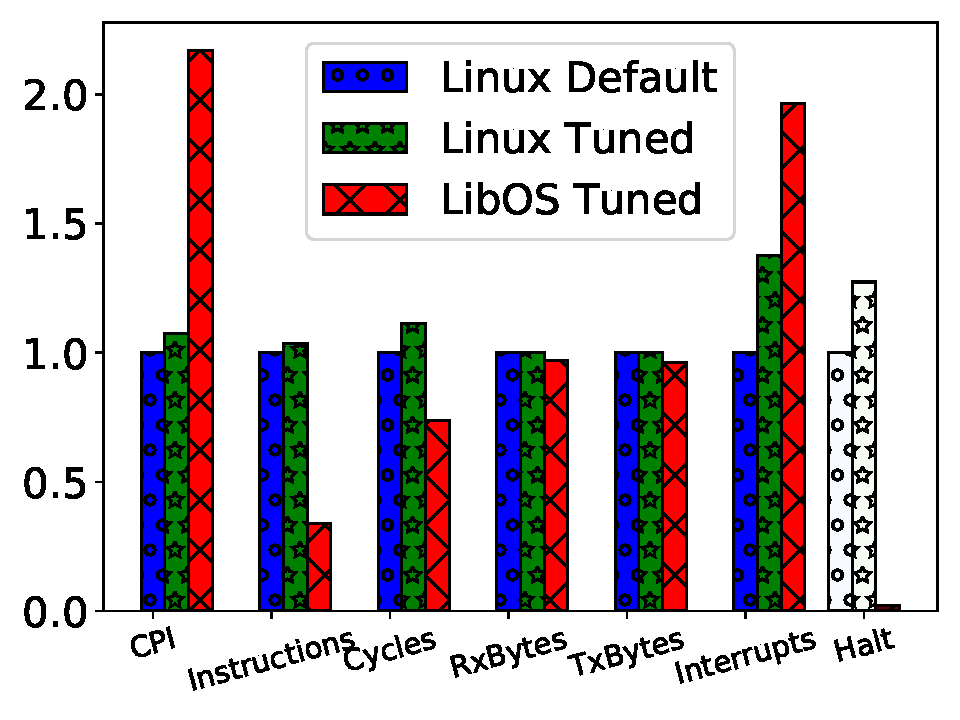
\includegraphics[width=\columnwidth]{osdi_figures/netpipe_65536_barplot}
        \end{subfigure}
 %       \hfill
        \begin{subfigure}[b]{0.35\textwidth}  
            \centering 
            \caption[]%
            {{Memcached:600K QPS}} 
            \vspace*{-0.3cm}    
            \label{fig:metrics_mcd600}
            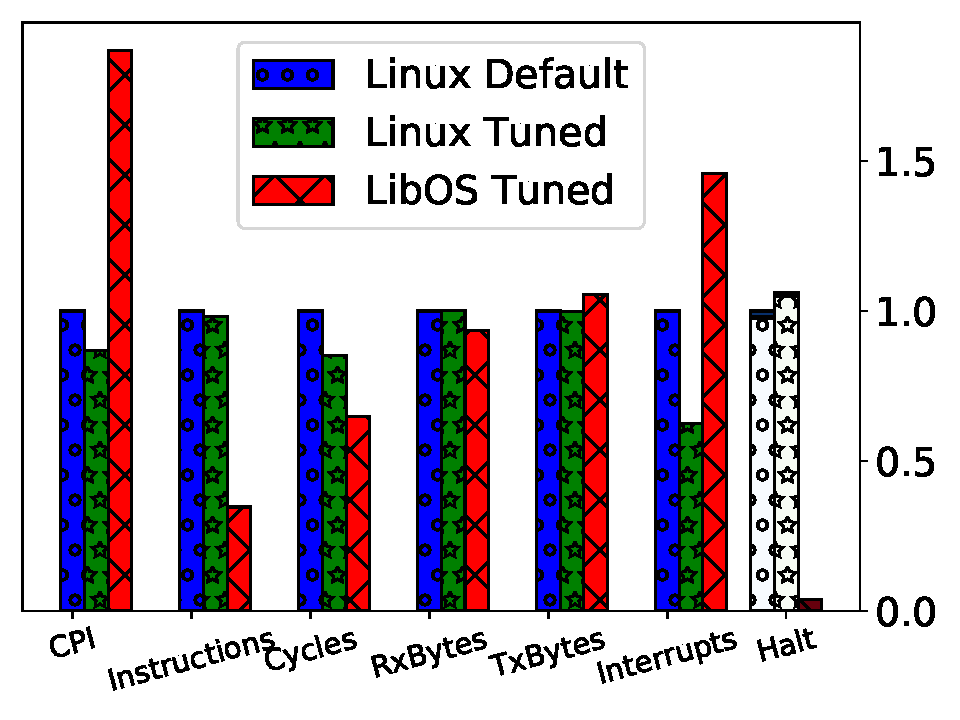
\includegraphics[width=\textwidth]{osdi_figures/mcd_600000_barplot}
        \end{subfigure}
        \vskip\baselineskip
        \vspace*{-0.4cm} 
        \begin{subfigure}[b]{0.35\textwidth}   
            \centering 
            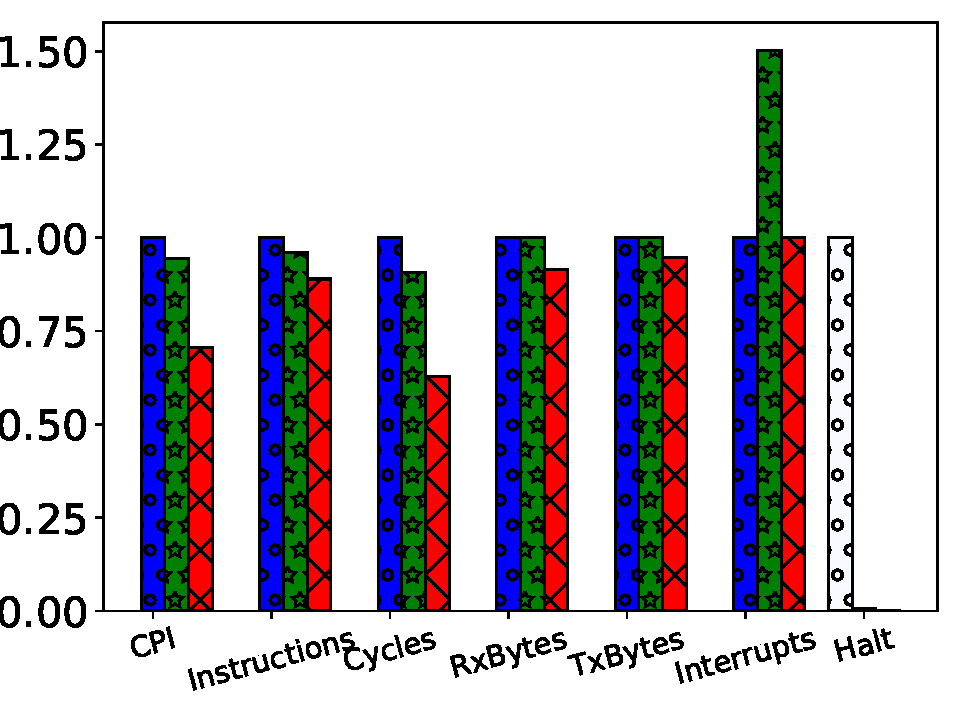
\includegraphics[width=\textwidth]{osdi_figures/nodejs_barplot.pdf}
            \caption[]%
            {{NodeJS}}    
            \label{fig:metrics_nodejs}
        \end{subfigure}
 %       \hfill
        \begin{subfigure}[b]{0.35\textwidth}   
            \centering 
            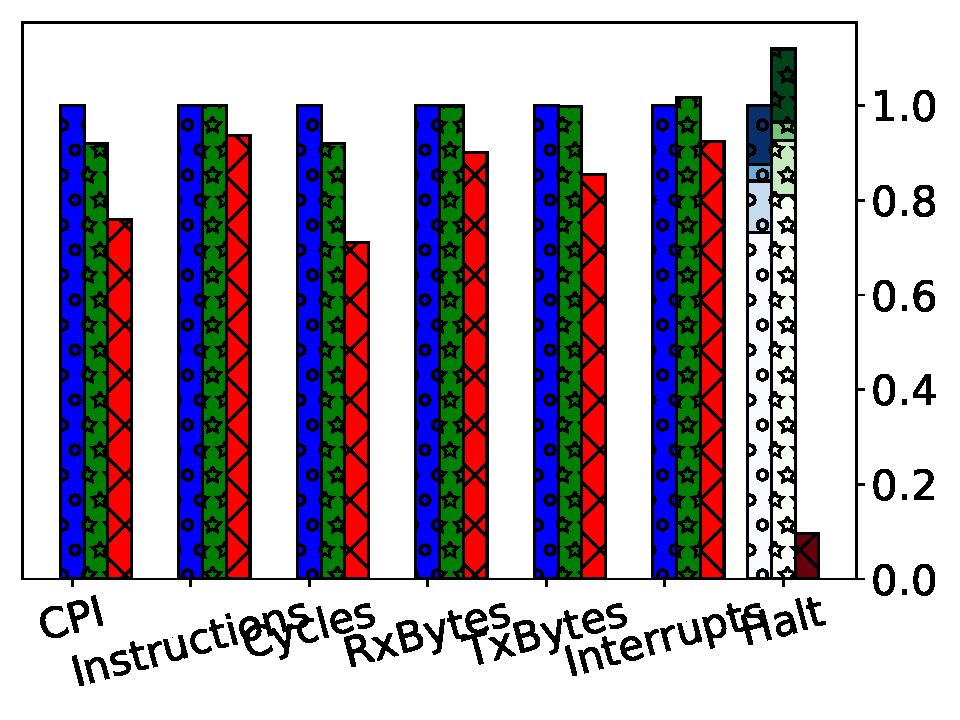
\includegraphics[width=\textwidth]{osdi_figures/mcdsilo_200000_barplot}
            \caption[]%
            {{Memcached-silo:200K QPS}}    
            \label{fig:metrics_mcdsilo200}
        \end{subfigure}
        \caption[]
        {Aggregate metrics from selected runs normalized against Linux default: For each experimental run, we instrument a detailed log entry collection in order to capture a set of hardware and software statistics. The halt bar shows the set of sleep state counts from C1 (lightest color) to C7 (darkest color) stacked on top of each other. %Each bar plot is a summation of all entries for that value in the per-interrupt log. 
        %Instructions and (unhalted) cycles are measured at a 1 ms timescale from reading Intel's PMC registers. Receive and transmitted bytes are read from the NIC's device driver data structures. The number of interrupts is measured as the length of all entries in a single experimental log. The halt bar shows the set of sleep state counts: [\texttt{C1}, \texttt{C1E}, \texttt{C3}, \texttt{C6}, \texttt{C7}], in Linux they are read from a the idle scheduler's data structure and in the libOS we keep a global counter before every \texttt{halt} instruction is called. 
        }  
        \label{fig:metrics}
    \end{figure*}%    
